\documentclass{beamer}

%\usepackage{beamerthemesplit}
\usepackage{beamerthemeshadow}
\usepackage[utf8x]{inputenc}
\usepackage[vietnam]{babel}

\title{\#CodingDojo @ Hanoi \\ Kata: Game of Life}
\author{Serge Stinckwich \& Dương ``Yang'' Hà Nguyễn}

\begin{document}

\maketitle

\frame{\tableofcontents}

\section{Introduction}

\frame{
  \begin{center}
    \textbf{\Huge What is the Game of Life?}
  \end{center}
}

\frame{
  \frametitle{What is the Game of Life?}

  \begin{itemize}
  \item<1->A board game!
  \item<2->Zero-player
  \item<3->$\rightarrow$ No winners
  \item<4->$\rightarrow$ No fightings
  \item<5->$\rightarrow$ Neat and safe!!!
  \item<6->Very simple rules.
  \end{itemize}
}

\frame{
  \frametitle{The Board}

  \begin{itemize}
  \item<1-> 2-dimensional grid of cells.
  \item<2-> Like this: \\
    \begin{center}
      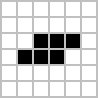
\includegraphics{goltoad1.jpg}
    \end{center}
  \item<3-> See the black and white cells?
  \item<4-> Black cells are alive ones.
  \item<4-> White cells are dead ones.
  \end{itemize}
}

\frame{
  \frametitle{Game Rules}

  \begin{itemize}
  \item<1-> Any living cell with fewer than 2 living neighbours dies
    (poor thing, caused by underpopulation).
  \item<2-> Any living cell with more than 3 living neighbours dies
    (caused by overcrowding).
  \item<3-> Any living cell with exactly 2 or 3 living neighbours lives
    on to the next generation.
  \item<4-> Any dead cell with exactly 3 living neighbours comes back
    to live.
  \end{itemize}
}

\frame{
  \frametitle{Like this}

  \begin{center}
    After one step, the board would transform like this (left to
    right): \\
    ~ \\
    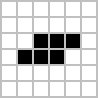
\includegraphics{goltoad1.jpg} ~~ 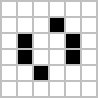
\includegraphics{goltoad2.jpg}
  \end{center}
}

\section{Problem Description}

\frame{
  \frametitle{The Problem}

  \Large Giving a board with finite dimensions.  Find the next
  transformation of the board after one step.
}

\frame{
  \frametitle{Data}

  \begin{columns}[c]
    \column{2in}
    \textbf{Input} \\
    \begin{itemize}
    \item<1-> $1^{st}$ row: Number of rows and columns, respectively.
    \item<1-> From $2^{nd}$ row: the board, ``$*$'' denotes living cells,
      ``$.$'' denotes dead cells.
    \end{itemize}
    Like this: \\
    \begin{center}
      \texttt{
        4 8 \\
        ........ \\
        ....*... \\
        ...**... \\
        ........
      }
    \end{center}

    \column{2in}
    \textbf{Output} \\
    The result board. \\
    ~ \\
    ~ \\
    ~ \\
    ~ \\
    ~ \\
    ~ \\
    Like this: \\
    \begin{center}
      \texttt{
        ........ \\
        ...**... \\
        ...**... \\
        ........ \\
      }
    \end{center}
  \end{columns}
}

\section{Solving with Randori}

\frame{
  \frametitle{Solving Game of Life with Randori}
  \begin{itemize}
    \item<1-> Writing tests first.
    \item<2-> Thinking (critically).
    \item<3-> Being a pilot/co-pilot and getting help.
    \item<4-> Don't forget to have fun!!!
  \end{itemize}
}

\frame{
  \begin{center}
    \textbf{\Huge Let's do it!!!}
  \end{center}
}

\frame{
  \begin{center}
    \textbf{\Huge Thank you for your attention!}
  \end{center}
}

\end{document}

%%% Local Variables: 
%%% mode: latex
%%% TeX-master: t
%%% End: 
